\documentclass[output=paper,english,spanish,german,english]{langsci/langscibook}
\ChapterDOI{10.5281/zenodo.4450085}

\author{Mario Bisiada\affiliation{Universitat Pompeu Fabra}}

\title[How \#MeToo is framed differently in Twitter discourse across languages]{Movement or debate? How \#MeToo is framed differently in English, Spanish and German Twitter discourse}

\abstract{This article examines 1,353 tweets on \mt in English, Spanish and German from July and August 2019, revealing how \mt is most commonly referred to as a \enquote{movement} in English and Spanish but as a \enquote{debate} in German, a difference that echoes German-language press habits. Based on an analysis of semantic prosody, the study demonstrates that words indicating longevity such as \enquote{era} and \enquote{times} collocate with \mt in English and Spanish, but not in German. This points to a framing of \mt as influential and long-term in English and Spanish and as exaggerated and short-term in German. Reflecting this difference, \mt is talked about in more negative terms in German tweets compared to English and Spanish, as shown by a qualitative analysis of evaluative author stance. The study adds to existing knowledge of the power of hashtags for feminist social media activism by highlighting the importance of (cross-)linguistic corpus-assisted discourse studies of hashtags on social media, which helps understand the ways in which anti-feminist discourse taps into the channelling of emotions through hashtags to undermine cross-national women’s movements.}
\glottocodes{stan1295,stan1288,stan1293}
\begin{document}

\maketitle

\section{Introduction}

Since it began trending in October 2017, the \mt hashtag has circulated in 85 countries \parencite[1317]{gilorg18} and has had a large-scale global impact on societies \parencite{zardav18}, both in terms of positive effects \parencite{fillon19} and backlashes \parencite{boyrat19}. Two thirds of Canadians say the \mt campaign has had an impact on them personally \parencite{reid18}. Consequently, there is a sizeable amount of literature on the hashtag's power for social movements and on its political effects, and some cross-cultural work has comparatively analysed attitudes towards \mt in the US and Norway \parencite{kunetal18} and investigated differences in media framing of women as \enquote{silence breakers} in the US, Japan, India and Australia \parencite{staetal19}. Linguistic studies of hashtags have mainly concentrated on functional aspects \parencite[see][7]{zappavigna18}, but cross-linguistic studies of hashtag use are still rare. Given that hashtags are usually transnationally used, studies of their effect on societies from a cross-linguistic and cross-cultural perspective could aid in the understanding of international hashtag activism, especially as regards the increasing global cooperation of feminist movements \parencites{huelga}{oppenheim18}[186]{garhop19}.

This paper analyses the framing of and evaluative stance towards the \mt hashtag from a cross-linguistic point of view to see how discourses around what seems to be the same concept diverge across languages and which effect this may have on language users' perception of the issue. Based on a corpus of English, Spanish and German tweets from July and August 2019, I address the following three research questions:

\begin{enumerate}
  \item How is the \mt hashtag represented in English, Spanish and German discourse through words that frequently accompany it?
  \item Which types of evaluative stance towards \mt can be identified and how do they differ cross-linguistically?
  \item Are there cross-linguistically similar discourse patterns around the \mt hashtag and what effect does this have on it as a safe space for hashtag feminism?
\end{enumerate}

\noindent While hashtags are generally agreed to empower women and feminist discourse on social media, some research has also questioned whether hashtag discussions really provide safe spaces. The core purpose of this paper is to demonstrate how linguistic analysis of hashtag discourse can identify reasons why hashtag networks are not always the safe spaces that hashtag feminism makes them out to be because they also allow or even attract misogynists to link into those networks. In the following section, I provide an overview of those arguments and discuss the importance of the study of hashtags as linguistic items.

\section{Communicative effects of feminist hashtags}\label{comm}

A major aim of hashtag activism has been to lay claim on public spaces \parencites[63]{luemai13}{bowles15}. Considering them a \enquote{collectivising feminist response to rape culture}, hashtags such as \#safetytipsforladies reveal \textcquote[354]{rentschler15}{the feminist delight in exposing misogynist, victim blaming ideas through humor}. Hashtag activism on social media plays an important role to establish counter-narratives against the dominating forces in public discourse. The hashtag \#MuslimWomensDay, for instance, gave Muslim women a voice to tell their stories and thus allowed them to challenge dominant media frames representing them as silent victims \parencite[200]{pennington18}. Other hashtags such as \#YesAllWomen and \#YesAllWhiteWomen created \enquote{feminist counterpublics} to \textcquote[392]{jacban16}{rewrite dominant public narratives about violence against women}.

Hashtags are powerful communicative and political tools because they allow victims of abuse to express and share their experiences and because they seem to affect people on an emotional level inaccessible to newspaper reports \parencites{keletal18}{menetal18}. Both of those capabilities make them more effective than traditional media and both can be traced to the combination of linguistic metafunctions that hashtags convey \parencite[see][]{zappavigna15}. The ability to evoke the appropriate emotions at particular moments in time and to control and channel these emotions is important in gaining followers for political movements \parencite{ahmed04}. This power can of course be used for both liberal and repressive campaigns, as the hijacking of \mt by far-right supporters such as the \#120dB campaign shows \parencites{farris17}{sorce18}{wielens19}.

Twitter enables girls and women to connect to each other and to share experiences of gender violence in hitherto unknown ways \parencite{keletal18}, bypassing the traditional news cycle and \textcquote[342]{williams15}{the mainstream media’s problematic framing of sexual violence and black women}. Participants in a study on the \#BeenRapedNeverReported hashtag \parencite{keletal18}, for instance, were reluctant to speak to the researchers and regarded Twitter as a safer way to share experiences of gender violence. The tweets \blockcquote[27]{keletal18}{all carried the common theme that it remained professionally, emotionally, and even physically costly to report sexual violence to authorities, disrupting the prevalent myth that unreported assaults are illegitimate}. The hashtag thus produced the benefit of giving its users a sense of community, affective solidarity and support \parencite[28--29]{keletal18}.

\newpage
In this way, hashtags have the political effect of creating new followers for the international feminist movement \parencites{schwin05}[238]{menetal18}. In her study of \#WhyIStayed, \textcite[789]{clark16} argues that the political effect hashtags have is caused by their ability to turn individual stories into a narrative, drawing on the feminist movement's historical emphasis on discourse, language and storytelling, while also enabling women to engage in \textcquote[796]{clark16}{dark parody of mainstream media discourse}.

\textcite{clark19} investigates activists' strategies to achieve visibility in a corpus of around 3,000 tweets using the \mt hashtag. She finds four major categories \parencite[7]{clark19}: 

\begin{enumerate}
  \item participants’ understandings of the political potential of \mt
  \item their takes on the tactic’s political limitations along with their attempts to redress these shortcomings
  \item their concerns regarding whose voices are included in the campaign
  \item their efforts to support the campaign and protect its survivor-participants
\end{enumerate}

\noindent She concludes that participants in \mt \textcquote[16]{clark19}{reclaimed their agency and pushed back against discourses that normalise harassment and assault}. The narratives collected under \mt have had the effect of a social transformation by making the personal political and scaling up from individual to collective visibility \parencite[16]{clark19}. Her study shows that sizeable participation is required to avoid that transgressions reported under a given hashtag become personalised or framed as individual errors, something that traditional media still tend toward \parencite[383]{kornemann18}. If it reaches sufficient participation, \blockcquote[16]{clark19}{the networking functions of the hashtag bridge the personal and the political, recasting, in the case of \#MeToo, sexual violence as a systemic, rather than private, issue and calling for structural changes in response}.

The advantages of hashtags over traditional media may well cause unease in the latter. Research has argued that media focus on celebrity involvement \textcquote[17]{banet18}{distract[s] us from systemic, structural sexism across all industries}. The hashtag \#Aufschrei (`outcry'), highly influential in Germany \parencite[see][]{maisch14}, has set the agenda in the public debate on sexism in spite of a largely antipathetic media focus \parencite[381]{kornemann18}. Traditional media have preferred to treat the \#Aufschrei movement in a symbolic way rather than engage with its content, thus reducing the general problem of gender discrimination to isolated occurrences \parencite[386]{kornemann18}. Such an approach \blockcquote[17]{banet18}{can end up working against the calls for social change promised at [the movement's] beginning, producing more and more visibility -- and increasingly narrowing the discourses of that visibility in the process}.

That individualising tendencies in reporting de-politicise feminist movements for their readership is also argued by \textcite[733]{benetal19} in their study of reporting on \mt in 613 UK newspaper articles from October 2017 to March 2018. Although they find that the press in the UK has played an important role in promoting \mt overall, they identify a focus on the stories of \enquote{the \enquote{ideal victims}, namely, celebrity female subjects (who are predominately White and wealthy)}, concluding that, \blockcquote[734]{benetal19}{by failing to inform the public about or to debate potential solutions, the press can be understood to have helped defuse any potential that \#MeToo might contain as a mobilising social force. Rather, the press seems to have framed \#MeToo largely in terms of neoliberal and popular feminisms, which disavow structural analysis and critique and largely place responsibility on individual women.}

\noindent Once a hashtag has firmly entered the public debate through mainstream media, it also becomes open to attacks by opposing forces. Based on a corpus of 700 tweets from between January 2013 and March 2014, \textcite{druzob16} analyse author stances towards \#Aufschrei, establishing the four categories of \enquote{supportive}, \enquote{neutral}, \enquote{dismissive} and \enquote{impossible to specify} \parencite[43]{druzob16}. They find that, from the second week onward, the supportive tweets increased and thus emphasised the importance of the hashtag \parencite[44--45]{druzob16}. The more widespread the hashtag became, however, the more it attracted dismissive reactions, and the personal experience postings were joined by blatant anti-feminist statements \parencite[44--45]{druzob16}. They conclude that Twitter cannot be considered a safe space, as \textcquote[51]{druzob16}{anti-feminist and sexist comments are equally visible and might signify new experiences of violence for women}.

The channeling emotional effect of hashtags may, then, also work the adverse way once abused by trolling or hate speech. The categorising function of the hashtag does not offer a filter to only encounter posts true to the original intention of the hashtag, which may have undesired consequences for social media users who find themselves in an emotionally fragile state induced by following the hashtag narratives. The power of hashtags is enhanced by \textcquote[652--653]{ging17}{the transnational nature and technological affordances of social media, whereby interest groups with similar agendas can more easily find one another}.

The study of hashtags unavoidably touches on the study of anti-feminist discourse on social media, which is transnationally networked and may share a set of cross-linguistic frames to attack feminist movements. That discourse is just the publicly visible face of a clandestine, globally networked subculture of men who describe themselves as \enquote{incels} \parencite[`involuntary celibates', see][]{valens18} and engage in celebrating violence against women and fostering a misogynist discourse on forums such as 4chan and 8chan \parencite[see][]{jaketal19}. These networks are a grave international threat: the terrorist attack in Christchurch (New Zealand) inspired men to commit similar attacks in Poway (US), El Paso (US), Baerum (Norway) and most recently Halle (Germany). In all cases, the shooters were regular users of 4chan or 8chan and explained their ideology in manifestos uploaded to those networks. In those manifestos, the terrorists express anti-semitic and white supremacist fears of white genocide through a decrease in fertility rates of white people, something for which they blame what they perceive as mass-immigration, but ultimately also feminism \parencites{distefano19}{kahsha19}.

These shootings are generally attributed to racist and anti-semitic views, while misogynist motives, though demonstrably present, tend to be ignored. Mass shooters are not necessarily all far right; the perpetrator of the 2019 Dayton shooting, probably inspired by the El Paso shooter, declared himself left-wing. What united him with the other shooters was that he showed signs of misogyny \parencite{svokos19}. In fact, \textcite{folexs19} show that in 22 analysed mass shootings since 2011, a third of perpetrators had a history of stalking and harassment and half of them specifically targeted women.

To understand how transnational, cross-linguistic misogynist and anti-fem\-i\-nist discourse works to globally attract particular groups of men, more linguistic research into its surface form on social media and hashtag discourse can be instructive. Hashtags are by necessity cross-linguistic phenomena; however, little cross-linguistic research on hashtags exists to date. Translation studies and corpus-assisted cross-linguistic discourse studies are fields that can contribute such analyses, and this chapter suggests one possible way of doing so through corpus study of semantic prosody and author stance. In the following section I outline how this study seeks to contribute such an analysis.

\section{Methodology}\label{sec:meth}

This study is based on 1,353 tweets containing the \mt hashtag (505 in English, 405 in Spanish and 443 in German), gathered between July and August 2019. The data were collected using the Twitter Search API. This API allows researchers to search for particular queries over a specific time period, within seven days of the tweet being posted. The API therefore gives us a snapshot view of the posts containing, in this case, the \mt hashtag at the present moment. It is important to note that the API is programmed by Twitter to not yield all the tweets containing this hashtag, but just a selection of what it considers relevant at the moment of searching \parencites[see also][7]{zappavigna18}{boyrat19}. The data analysed here should thus be understood as a snapshot comparison of activity around the \mt hashtag in the English, Spanish and German language communities\footnote{In this paper, I refer to language communities instead of countries for two reasons, which I think apply generally to cross-linguistic studies of social media data. First, the internet is a transnational space, so discussions happen within language communities, which often transcend countries. Secondly, the country stated in the profile (if at all) does not allow us to make inferences on the native language of the user.} during July and August 2019.

One important aspect in the analysis of collocations across languages is the difference in how lexical units are usually formed. Spanish uses slightly different word formation rules to English and German; while it is \textcquote[81]{lang90}{somewhat resistent to orthographic noun compounds}, typical in Germanic languages, the more natural and \textcquote[85]{lang90}{highly productive} construction in Spanish would be what \textcite[85]{lang90} calls \enquote{prepositional link syntagms}, where words are joined with the preposition \textit{de} (in our case \textit{x de(l) \#MeToo}) to form a lexical unit \parencite[85]{lang90}. Not taking this difference into account may well lead to observing a higher likelihood of collocations in English and German compared to Spanish. Therefore, I have decided to count such prepositional link syntagms, which also occur in the Germanic languages, albeit at a lesser rate, among the collocations. Here is an example of one such prepositional link syntagm:

\begin{quote}\sffamily
  En la era del \#metoo este rollo de mujer objeto del desfile de Victoria's Secret se ha quedado obsoleto, y a la gente joven les parece casposo. No veo la mala noticia por ningún lado.\newline [`In the \mt era, this whole thing of objectifying women that is the Victoria's Secret fashion show has become obsolete and to young people it seems inappropriate. I don't see the bad news at all.']
\end{quote}

\noindent While the Twitter Search API gives access to the username of the author of the tweet, I have anonymysed all usernames mentioned in the examples to \enquote{@user}, except institutions or public figures, defined as those with verified accounts \parencite{twitter19}. Images in the tweet and retweets of other tweets are converted to abbreviated links by the Search API, in addition to links the user may have posted. While the analysis of author stance has taken into account the entire tweet including images and articles linked to, I have generally removed all links from the tweets printed as examples in this paper in order to remove visual clutter. The tweets are not otherwise edited for orthography and all translations are my own. I have made the data underlying this research open and encourage readers wishing to consult the full tweets to do so. % cite link to open data

As stated above, the objectives of this study are to analyse the semantic pros\-o\-dy of \mt in Twitter discourse and to investigate the author stance in the tweets where the \mt hashtag is integrated into the sentences. Semantic prosody is here understood as pragmatic colouring applied to words by its collocates \parencites[158--159]{louw93}{stewart10}[13--14]{vessey13}, a concept that has proved useful also in cross-linguistic research \parencite{lewandowska96}. I am here specifically interested in what \textcite[61]{stewart10} terms the study of semantic prosody as a feature of word + co-text, by which \textcquote[61]{stewart10}{some lexical items are associated with prosodies whose meaning is in marked contrast with the basic meaning of the node\slash core item in question}. We can extend this notion to the case where a new hashtag such as \mt is integrated into a compound and thus given a particular colouring through the semantic prosody of the accompanying term. Crucially, I adopt the view that \textcquote[13]{vessey13}{through his or her language, and more specifically, through the use of collocations and the effect of semantic prosodies, an acculturated speaker often (re)produces the values and judgments of his or her discourse community}. In the present context, I argue that the collocates appearing alongside \mt allow us to discern the stance towards the issue prevalent in each respective language community.

For the analysis, I have first separated those tweets where the hashtag is part of the sentence like any other word from those where it is put at the end, outside the sentence. In the former case, it is said to serve as a lexical item in \enquote{integrated} position, while in the latter, the hashtag is in \enquote{culminative} position \parencites[31--32]{zappavigna18}[see also][14]{scott15}. Hashtags in the integrated position \textcquote[32]{zappavigna18}{take on functional roles in the clause. In culminative position, while the hashtag can construe any number of functional roles on its own \textelp{}, it is typically not integrated into the clause. Instead it is appended at the end of the post}.

To analyse semantic prosody of the \mt hashtag, then, the first step is to separate occurrences according to this criterion, as well as to mark duplicate tweets, which mainly include newspaper headlines shared by many people, and unrelated uses of the hashtag, mainly to say \enquote{me too} without referring to the movement. Each hashtag integrated into the sentence is then analysed to see if it appears as a collocation and, if so, which collocate accompanies it.

To address the second research question, the analysis of author stance, I have conducted an analysis of tone using the method proposed by \textcite{orgben15} and \textcite{druzob16}. Thus, tweets were considered \enquote{positive} if they showed \enquote{commendation\slash appraisal\slash valuing\slash appreciation or recognition} of \#MeToo, and \enquote{negative} \textcquote[424--425]{orgben15}{if they demonstrated or included substantial criticism\slash derision\slash cynicism or dismissal} of \#MeToo. In addition, I have established the category \enquote{critical} for tweets that criticise \mt in a constructive way, expressing discontent with some aspect but being in favour overall. Tweets that cannot clearly be attributed to any of these categories have been labelled \enquote{unclear}.

For the final objective, the identification of cross-linguistic framings, I have compared the findings from the first research question and compared the semantic prosodies identified for each language in order to identify patterns.

\section{Semantic prosody of \#MeToo}\label{pros}

\begin{table}[b]
\caption{Absolute (n) and relative (p) frequencies of occurrences of the \mt hashtag in the corpora of tweets}\label{freq}
  \begin{tabularx}{\textwidth}{X rr@{\qquad}rr@{\qquad}rr}
    \lsptoprule
    \textbf{Category}    & \multicolumn{2}{c}{\bfseries English} & \multicolumn{2}{c}{\bfseries Spanish} & \multicolumn{2}{c}{\bfseries German}\\
                    & n   & p                     & n   & p                     & n   & p\\
    \midrule
    integrated      & 210 & 41\%                  & 237 & 58\%                  & 184 & 41\%\\
    external        & 242 & 47\%                  & 126 & 31\%                  & 202 & 46\%\\
    unrelated       & 18  & 4\%                   & 10  & 3\%                   & 13  & 3\%\\
    duplicate       & 41  & 8\%                   & 32  & 8\%                   & 46  & 10\%\\
    \midrule
    \textbf{Total}  & 511 & 100\%                 & 405 & 100\%                 & 445 & 100\%\\
    \lspbottomrule
  \end{tabularx}
\end{table}

Table~\ref{freq} shows the absolute and relative frequencies of \mt hashtags that are in the integrated and in the culminative position, as well as unrelated and duplicate occurrences. In English and German, 41\% of the tweets have the hashtag in integrated position while about half of all occurrences are culminative. In Spanish, 60\% of the hashtag occurrences are integrated while only about a third are culminative. This may indicate a preference on the part of Spanish users to integrate the hashtag into the sentence, though a larger corpus sample is necessary to support this observation. Based on these data, I have proceeded with analysing the semantic prosody of the \mt hashtag.


\noindent To analyse the semantic prosody of the \mt hashtag, I have conducted a frequency analysis of its collocations where it does not occur as a single word. There are five occurrences of a verb form \textit{metoo'd}, a verbalisation that is interesting from a formal linguistic point of view and a commonly observed phenomenon in English, but need not concern us any further at this point. I have counted these occurrences among the single-word occurrences. The absolute and relative frequencies of \mt as a single word are as follows:

\begin{description}
  \item[English] 83 single-word occurrences (40\% of the integrated occurrences)
  \item[Spanish] 143 single-word occurrences (60\% of the integrated occurrences)
  \item[German] 114 single-word occurrences (62\% of the integrated occurrences)
\end{description}

\noindent This means that in English, a slight majority of the hashtags in integrated position are parts of collocations, while in Spanish and German, single-word occurrences are in the majority. While this may indicate a slight preference among English users to form collocations with the \mt hashtag when compared to Spanish and German users, this quantitative observation again needs to be backed up by a larger data sample. Table~\ref{coll} shows all the collocates of the \mt hashtag found in the corpora, with the number of occurrences in parentheses. I now discuss the three corpora in turn.

\begin{table}
  \caption{Collocates of \mt in the English, Spanish and German corpora, sorted by frequency of occurrence (single-occurrence items omitted)}\label{coll}
  \begin{tabularx}{\textwidth}{l@{~}p{0.27\linewidth}p{0.32\linewidth}Q}
    \lsptoprule
        & \textbf{English} (n=127) & \textbf{Spanish} (n=94) & \textbf{German} (n=70)\\
    \midrule                                                                              
    1.  & movement (38)
        & movimiento (44)
        & Debatte (16)\\
    2.  & moment (15)
        & tiempos (9)
        & Hysterie (8)\\
    3.  & campaign (8)
        & era (6)
        & Bewegung (6)\\
    4.  & era (7)
        & campaña (4)
        & Aktivistin(nen) (`activist(s)' (f.)) (3)\\
    5.  & merch, case (3)
        & momento (`moment') (2)
        & Hexenjagd (`witch hunt'), Kampagne (`campaign'), Inquisition, Zeiten (`times'), Befindlichen (`affected'), Folgen (`consequences') (2)\\
    6.  & accusers, complaints, rhetoric, story, survivor, victims (2)
        & 
        & \\
    %7.  & age, bitches, mass-emasculation, drama artists, allegations, violations, leadership, supporter, phenomena, rebellion, architect, hot mess, concerns, incident, nutcase, madness, outfits, hashtag, battle, crimes, claim, thing, idea, path, BS, coverage, false accusations, gang, helpline, issues, legal advice, memo, news, paranoia, reporting, world (1)
    %    & {\small chilladeras (`outbursts'), marca (`brand'), camino (`path'), caso (`case'), época (`epoch'), carro (`bandwagon'), jevitas (`sexy girls'), iniciativa (`initiative'), fetiche (`fetish'), compromiso interinstitucional (`inter-institutional commitment'), mundo (`world'), compromiso internacional (`international commitment'), trama (`narrative'), acusados (`accused'), feministas (`feminists'), agendas (`agendas'), contexto (`context'), acusaciones (`accusations'), declaraciones (`reports'), efectos (`effects'), euforia (`euphoria'), totalitarios del feminismo (`feminist totalitarians'), veda (`hunt'), mujeres (`women'), red internacional (`international network'), hashtag, pantalleras (`attention-seekers'), discursos (`discourses'), fenómeno (`phenomenon')} (1)
    %    & Sexualhexenjagd (`sexual witch hunt'), Diskurs (`discourse'), Falschbeschuldigung (`false accusation'), Lynchmob, Hype, Zug (`train'), Sturm (`storm'), Welle (`wave'), Argumentation, Unsinn (`nonsense'), Kartenhaus (`house of cards'), Gschichtli (`little story'), Dorf (`village'), Outerinnen, Tanten (lit. `aunts', derog.), Betroffene (`affected'), Post (`post'), Faktor (`factor'), Opfer (`victim'), Vorwürfe (`accusations'), Gegenwart (`present'), Beschuldigte (`accused'), Brigade, Movement, Studie (`study') (1)\\
    \lspbottomrule
  \end{tabularx}
\end{table}

\subsection{The English corpus}

In the English corpus, the most common collocate with 38 occurrences is \textit{movement}, exemplified below.

\begin{quote}\sffamily
  The theme of gender oppression runs throughout the collection, as befits current debates in the West and beyond over sexual violence and predatory behaviour in the wake of the \#metoo movement.
\end{quote}

\noindent This collocate is supported by the fact that \mt is now labelled a movement on Wikipedia and that there is an official movement page offering \blockcquote{metoo}{a comprehensive database consisting of local and national organisations dedicated to providing services and safe spaces for survivors of sexual violence, healing stories, as well as articles and a glossary of terms to help give voice to your experiences}. While it is a neutral term in that it does not in itself show positive or negative stance, its use does mean a recognition of the hashtag as influential and with potentially large-scale effects on society, which gives the compound \textit{\#MeToo movement} an approving stance.

The collocation \textit{moment} occurs 15 times, mainly in tweets citing some entity's \mt moment, as in the first example below, but it can also denote just a momentary instance of something bigger, as in the second example:

\begin{quote}\sffamily
  .@ruthmaclean reports on how `Nigeria's \#MeToo moment' turned against rape accuser \#globaldev
  
  A definite \#MeToo Moment. I'm retweeting because she shouldn't be the one quitting. These people should be reprimanded and forced to pay restitution. The Rookie production should be behind her.
\end{quote}

\noindent As a collocation, \textit{\mt moment} is used as a label under which a series of articles as well as \enquote{updates and analysis on the \#MeToo movement} are collected in the New York Times \parencite{bennett19}. In fact, whether \mt is a movement or a moment has been discussed in a series of press articles \parencite{akhtar17} which argue that \textcquote{senecal18}{unless actions replace hashtags and value signaling, we'll see old power structures and patterns of behaviour remain as entrenched and unequal as ever -- along with a healthy new dose of mistrust and resentment with which women will contend}. Tarana Burke, the founder of the movement, has said in a TED talk in 2018 that the fact she is giving this talk shows that \mt \textcquote{burke18}{is bigger than a moment. It's the confirmation that we are in a movement. And the most powerful movements have always been built around what's possible, not just claiming what is right now}.

In a Canadian survey, a majority of participants consider \mt a movement, with 53\% of participants saying that \enquote{the \#metoo movement will lead to some change, but it will take years, if not decades for real change} and 31\% saying that \enquote{these discussions have sparked a major and permanent shift}, while only 14\% believe that \enquote{people might be paying attention now, but it will blow over, and nothing will really change} \parencite{reid18}. It is this last view of \mt that the \textit{moment} collocation arguably expresses, either out of sheer rejection of the movement or because its user accepts the systematicity of the transgressions, but does not have any hope that things will change.

With eight occurrences, we find the collocate \textit{campaign}, followed by \textit{era} with seven occurrences. The collocate \textit{campaign} in itself is a neutral term, similar to \textit{movement} in that it is a collective action, though not as widely influential as a movement. It was mainly used by the press in articles immediately after the initial wave of \mt postings and, as the examples show, might now be used by people who are critical of or reject the movement.

\begin{quote}\sffamily
  @therealaftonw if \#AftonWilliamson was lighter, blond haired, light eyed, pointy nosed then could she then be a part of the \#MeToo campaign? Investigate the matter please and get back to me

  The story of fake rape allegations against \#TonyMochama as found by our courts militate against the \#Metoo campaign turning the entire mass hysteria  on its head. Kindly guys its never worth it.... why cook a false narrative and drive it for sympathy and in the end tarnish ppl
\end{quote}

\noindent The word \textit{era} also denotes a time span and is thus comparable to \textit{moment}, though it has the added semantic shade of referring to a before and after of a certain watershed moment. As the examples show, it goes along with a certain desperation at a given event and seems to be used mainly to achieve a semantic prosody of indignation based on \#MeToo, without necessarily taking a stance towards the hashtag itself.

\begin{quote}\sffamily
  @user @brianefallon So drunk staff being inappropriate makes it OK for sobet teens to mime choking a young women in the \#MeToo era with rampant campus rapes?? I don't like Whataboutism \#STUPIDITY

  @user @user @brianbeutler In the very unlikely event he got the nomination, Bernie’s rape fantasy or teacher bashing essays will be widely disseminated by the GOP. I cannot, for the life of me, see how this isn't disqualifying in the \#metoo era.
\end{quote}

\noindent Many of the collocations used three times or less are rather self-explanatory rejections of the \mt movement and will not be commented on.

\subsection{The Spanish corpus}

Looking at the Spanish data, we find the collocate \textit{movimiento} (`movement') with 44 occurrences as by far the most frequent collocation, just as it is for the English data. The Spanish-language Wikipedia entry for \mt also describes it as a movement, and various Spanish language glossaries list the hashtag as a movement. The Spanish newspaper El País has featured a special entitled \textit{Revolución MeToo} \parencite{elpais18}, where \mt is either referred to without any collocates or as a movement. Here is an example illustrating the collocation:

\begin{quote}\sffamily
  \foreignlanguage{spanish}{@user Pues que ahora, gracias al movimiento  \#metoo se atreven a denunciar y a declarar en contra de esos antaño intocables y todopoderosos hombres que las han tratado como a cachos de carne de mercado desde su infancia.}\newline [`Well that now, thanks to the \#metoo movement, they dare to speak out and make a statement against these formerly untouchable and all-powerful men who have treated them like pieces of meat at a market since they were kids.']
\end{quote}

\noindent The second most common collocate in the Spanish data is \textit{tiempos} (`times') with nine occurrences, followed by \textit{era} (`era') with six occurrences, taking into account that this includes prepositional link syntagms (see the Methodology section). The word \textit{campaña} (`campaign') occurs four times. Below are some examples.

\begin{quote}\sffamily
  \foreignlanguage{spanish}{En la era \#MeToo, hay que convertir los espacios públicos en lugares donde las mujeres puedan existir sin ser miradas, juzgadas o comentadas}\newline [`In the \#MeToo era, public spaces must be converted to places where women can exist without being looked at, judged or commented on']

  \foreignlanguage{spanish}{A sumarnos a la campaña \#METOO por menos mujeres con violencia\newline Más mujeres felices\newline \#uniendofuerzas}\newline [`Let's join the \#METOO campaign for fewer women with violence [sic] --- more happy women --- \#unitingforces']
\end{quote}

\noindent The Spanish data thus largely mirror what has been observed in the English data.

\subsection{The German corpus}

The German data differ from the English and Spanish data discussed thus far in that \textit{Bewegung}, the German equivalent for \enquote{movement}, only occurs in six tweets, most of which attack the movement, as shown below.

\begin{quote}\sffamily
  \foreignlanguage{german}{@Junge\_Freiheit wie erwartet stellt sich in vielen Fällen heraus, dass diese \#metoo Bewegung eine inquisitorische Hexenjagd auf Unschuldige war\slash ist, was diese widerliche Bewegung 1.000 mal schlimmer macht als das was sie anprangert.}\newline [`as expected, in many cases it turns out that the \#metoo movement was\slash is an inquisitorial witch hunt for innocents, which makes this disgusting movement 1,000 times worse than that which it condemns.']

  \foreignlanguage{german}{@westfalenblatt Also DER \#Leuchtturm Fall der \#MeToo Bewegung steht auf so wa\-cke\-ligen Beweisen, dass der Fall eingestellt werden muss. Was ist denn dann mit den ganzen anderen Fällen, die nur in der \#Empörungswelle mitschwammen? Wer entschädigt jetzt diese Opfer, wo blieb die Unschuldsvermutung?}\newline [`So THE landmark case of the \#MeToo movement is based on such shaky evidence that the case has to be closed. What then happens in all the other cases that just joined the flow of indignation? Who will indemnify these victims, what happened to the presumption of innocence?']
\end{quote}

\noindent Interestingly, at the time of writing of this article, the German-language Wiki\-pe\-dia page does not define \mt as a movement, but just as a \enquote{hashtag}.

The most frequent collocate in the German data is \textit{Debatte} (`debate'), which occurs 16 times. As we saw above, this frame does not occur at all in the English and Spanish data. Below are some examples.

\begin{quote}\sffamily
  \foreignlanguage{german}{Schauspielerin Emilia Schüle findet die \#Metoo-Debatte wichtig---und dass sich in der Gesellschaft noch viel ändern muss.}\newline [`The actress Emilia Schüle considers the \#Metoo debate important---and that much still has to change in society.']

  \foreignlanguage{german}{Die \#MeToo-Debatte um Alltagssexismus hat einer Studie zufolge die Situation für Frauen am Arbeitsplatz in den USA leicht verbessert.}\newline [`The \#MeToo debate on daily sexism has lightly improved the situation of women in the workplace, according to a study.']

  \foreignlanguage{german}{@tazgezwitscher @user @user ohne, dass es Proteste gibt. Danke jedenfalls für den Einblick in die Blase des US-Feminismus. Vielleicht ist das das Problem bei der \#metoo Debatte in Deutschland, dass man auf Twitter unter \#metoo viel US-Feminismus mitbekommt, was nicht der Realität in Deutschland entspricht?}\newline [`without there being protests. Thanks anyway for the insight into the bubble of US feminism. Maybe that's the problem with the \#metoo debate in Germany, that you get a lot of US feminism under \#metoo on Twitter, which doesn't conform to the reality in Germany?']
\end{quote}

\noindent These are moderate comments on the topic, which shows that the word \textit{debate} is the common collocate used with \#MeToo in German. A query in the DWDS newspaper corpus, consisting of the most important German-language newspapers, confirms this impression: in texts from 2017 and 2018, where \#MeToo as a single word occurs 384 times, \textit{\#MeToo-Debatte} occurs 178 times, while \textit{\#MeToo-Bewegung} occurs 49 times \parencite{dwds}. It seems, then, that in German-language public discourse, the most common way to frame the \#MeToo hashtag is not as a movement, but as a debate, and that the press is actively involved in promoting this frame through the use of the term \textit{\#MeToo-Debatte}. It seems, then, that, while international discourse on \mt awards it the status of a movement and all the connotations of this as described above, German discourses avoid such a labelling for some reason.

This might be explained by a tendency among German media to envisage a hierarchical cline between traditional and new media, which affects their role in society and against which they seek to strengthen their own position \parencite[382]{kornemann18}. Hashtag movements such as \#MeToo, which enter public discourse as folksonomic creations having circumvented traditional news media gate-keepers, still leave the traditional media somewhat taken aback and struggling to react appropriately. This might be especially true of feminist movements, which meet strong hegemonic barriers through the patriarchal establishment and recurrent discrimination of women that still pervade many press agencies \parencite{banet18}. A possible explanation for the establishment of the more reluctant \enquote{debate} frame may thus be that labelling \mt a movement would distance traditional media from further involvement, while framing it as a debate means the traditional media retain an active role in its development.

The second most common collocate in German is \textit{Hysterie} (`hysteria'), with 8 occurrences, a purely negative frame which is not found in the English and Spanish data either. Its occurrence may have been pushed by a lot of activity around an influential blog article, which may have distorted the data somewhat, but this frame goes hand in hand with the intent to reclaim the term \textit{Opfer} (`victim') and apply it to those accused under the \mt hashtag, observable in a range of examples.

\begin{quote}\sffamily
  \foreignlanguage{german}{Anklage gegen Opfer der \#MeToo Hysterie wird fallengelassen.}\newline [`Case against victims of \mt hysteria is dropped.']

  \foreignlanguage{german}{Was von der \#metoo Hysterie blieb. Jetzt läuft die \#Klimahysterie. \#Fridaysforfuture \#Great \#Grüne \#Kulturbereicherung}\newline [`What remains of the \#metoo hysteria. Now it's the \#ClimateHysteria. \#Fridaysforfuture \#Great \#Greens \#CulturalEnrichment']
\end{quote}

\noindent Given the frequency in English and Spanish of terms such as \textit{era}, \textit{tiempos} or \textit{moment}, which frame \#MeToo temporally, as something that is long-term and influential, it is notable that the only collocate in the German corpus reflecting such a frame is \textit{Gegenwart} (`present'), and two tweets containing the phrase \textit{in Zeiten von \#MeToo} (`in times of \#MeToo'), as shown below. Again, a query in the DWDS newspaper corpus confirms the absence of this frame from German discourse, as, for instance, \textit{\#MeToo-Ära} occurs just three times \parencite{dwds}.

\begin{quote}\sffamily
  \foreignlanguage{german}{Lashana Lynch: Wie auch James Bond in die MeToo-Gegenwart gezerrt wird \#JamesBond \#MeToo}\newline [`How even James Bond is dragged into the MeToo present']

  \foreignlanguage{german}{@ulfposh Alter weißer Mann findet alten weißen Mann gut. Solidarität unter Privilegierten in Zeiten von \#MeToo, \#rechtsterrorismus und \#Frauenquote uvm nur logisch}\newline [`Old white man likes old white man. Solidarity among the privileged in times of \#MeToo, \#farrightterrorism and \#women'squota etc no surprise']
\end{quote}

To sum up, we can observe a notable difference between the English and Spanish language community on the one hand and the German language on the other just when it comes to the way \mt is referred to. While English and Spanish discourse generally award it the status of a movement and also use other, more appreciative collocations, German discourse is more reluctant and just labels it a debate, which has fewer empowering features than the term \textit{movement}. This may affect the degree to which \mt can be seen as a safe space for women participating in internet discussions surrounding the hashtag then.

It will be interesting to see whether this difference in how \mt is perceived on a general discourse level is also observable in individual author positions in the tweets. The second research objective is to conduct an analysis of author stance towards \mt in the English, Spanish and German tweets (see Table~\ref{tab-stance}, visualised in Figure~\ref{stance}). The tweets in the English and Spanish corpora show a higher frequency of positive stance (47\% and 42\%) when compared to the tweets in the German corpus (27\%), and show a lower frequency of negative stance (27\% and 29\%) than the German tweets (44\%). Keeping in mind that the sample size is not huge and provides just a snapshot of activity, the data seem to indicate that the general stance towards \mt is more negative in German Twitter discourse during the recorded time span than in English and Spanish.

\begin{table}[b]
\caption{Analysis of positive, critical, negative and unclear author stance in the three languages}\label{tab-stance}
  \begin{tabularx}{\textwidth}{lrrrrrrrrrr}
    \lsptoprule
            & \multicolumn{2}{c}{\bfseries positive}
                          & \multicolumn{2}{c}{\bfseries critical}
                                      & \multicolumn{2}{c}{\bfseries negative}
                                                    & \multicolumn{2}{c}{\bfseries unclear}
                                                                & \multicolumn{2}{c}{\bfseries total}\\
            & n   & p     & n   & p   & n   & p     & n   & p     & n   & p\\
    \midrule
    English & 98  & 47\%  & 8   & 4\% & 46  & 22\%  & 58  & 27\%  & 210 & 100\%\\
    Spanish & 100 & 42\%  & 17  & 7\% & 52  & 22\%  & 68  & 29\%  & 237 & 100\%\\
    German  & 50  & 27\%  & 17  & 9\% & 81  & 44\%  & 36  & 20\%  & 183 & 100\%\\
    \lspbottomrule
  \end{tabularx}
\end{table}

\begin{figure}[b]
  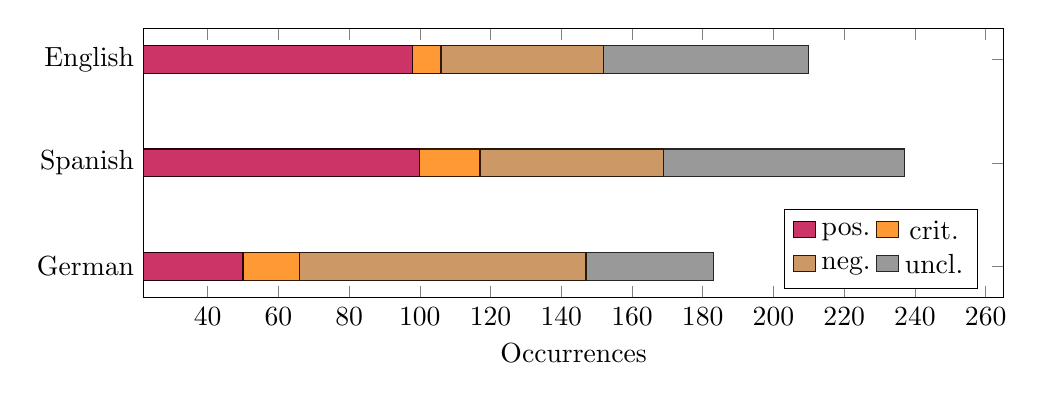
\begin{tikzpicture}
    \begin{axis}[
      xbar stacked,
      width=125mm,
      height=5cm,
      enlargelimits=0.15,
      legend pos=south east,
      legend columns=2,
      xlabel={Occurrences},
      symbolic y coords={German, Spanish, English},
      ytick=data,
      ]
      \addplot[purple!20!black,fill=purple!80!white] coordinates{
        (98,English) (100,Spanish) (50,German)
      };
      \addplot[orange!20!black,fill=orange!80!white] coordinates{
        (8,English) (17,Spanish) (16,German)
      };
      \addplot[brown!20!black,fill=brown!80!white] coordinates{
        (46,English) (52,Spanish) (81,German)
      };
      \addplot[lightgray!20!black,fill=lightgray!80!black] coordinates{
        (58,English) (68,Spanish) (36,German)
      };
      \legend{pos., crit., neg., uncl.}
    \end{axis}
  \end{tikzpicture}
  \caption{Graph of positive, critical, negative and unclear author stance in the three languages}\label{stance}
\end{figure}

The analysis thus suggests that in German-language Twitter discourse, contrary to English and Spanish-language discourse, the reluctance to call \mt a movement, or a lasting societal shift, but mainly a \enquote{debate}, is reflected in the general population's stance towards the hashtag and translates into a more negative attitude towards it, again putting into doubt whether the hashtag in German can be considered a safe space. Of course the use of the word \textit{debate} in itself, as the above examples suggest, does not necessarily imply negative author stance. It could be argued, however, that the prevalence of the \enquote{debate} frame has promoted a type of individualising tendency which, as pointed out by research discussed above, de-politicises the \mt movement. After all, a debate is understood as an open-ended discussion depending on individual views between at least two legitimate sides which have equal justification of existence. Given, however, that \mt was sparked by a series of revelations of sexual assault and developed into a movement to end gender violence in society, it is hard to see any justification for labelling it a \enquote{debate}. The often misogynistic and derisive statements we observe in this analysis, however, show that a less appreciative labelling of the hashtag accompanied by a largely negative discourse around it can endanger the perception of the hashtag as a safe space for feminist activism.

\section{Cross-linguistic framings of \#MeToo}

Having indicated differences between the languages under analysis, I now turn to the third research question, the analysis of cross-linguistic similarities. One representation that is obvious from the collocates identified in the previous analysis is that of \mt as a collection of lies, which is perhaps the most lexically creative attack on the movement. Beyond that, this section identifies two framings that language users in this corpus apply to \mt across languages: the \textit{organised pressure group} frame and the \textit{exaggerated scope} frame. I also discuss the hijacking of the movement by far-right groups.

The first frame that can be identified is that of \mt as an organised pressure group. A range of comments in the corpus suggest that commentators across languages treat \mt as a centrally controlled organisation:

\begin{quote}\sffamily
  @user @user @user @user The current \#MeToo leadership are mostly the men hating lesbians. They are desperately trying to create a wedge between men and women. Therefore anything men do to honour and please women must be attacked and denigrated.

  @user It specifically painted \enquote{hippie chicks} as childish, dirty, drugged out, homicidal morons whose violent deaths are to be celebrated. That had to upset more than one \#MeToo architect over at Alyssa Milano’s agency, CAA. After all, Tarantino is repped by WMA, their competitor.

  \foreignlanguage{spanish}{Lo que no entiendo es cómo, en el mismo mundo del movimiento \#MeToo y del poderoso lobby feminista -uno de los grupos de presión más poderosos de la actualidad-, todavía pueda existir el reggaeton}\newline [`What I don't understand is how, in this world of the \#MeToo movement and the powerful feminist lobby -one of the most powerful pressure groups of our time-, there can still be Reggaeton.']

  Wieder ein Opfer der totalitären \#MeToo-Inquisition, dessen Rehabilitierung am Ende mit einem Dreizeiler erledigt wird und der mit seinem sozialen und beruflichen Tod allein bleibt.\newline [`Another victim of the totalitarian \mt inquisition whose rehabilitation in the end is given short shrift and who remains alone with his social and professional death.']
\end{quote}

\noindent Words like \textit{architect}, \textit{leadership} and \textit{lobby} clearly show that these authors perceive \mt not as the decentralised popular movement against everyday gender violence that it is, but as an organised campaign attributed to left-wing lobbies, claimed to be funded by George Soros and led by a few activist women with the political goal to eliminate men who disagree, as evidenced further in the examples below.

\begin{quote}\sffamily
  @user @irlembberlin @bpol\_b Makes sense. Men are the key to the streets \& have been propaganda targeted by \#WhiteFeatherMedia \& political \#gaslighting; by \#MeToo mass-emasculation \& dehumanisation of men -- ready to *trigger* \& mobilise a global army...

  \foreignlanguage{german}{Was bleibt von \#metoo? -- die Motivation, politisch unliebsame Männer gesellschaftlich zu vernichten.}\newline [`What remains of \#metoo? -- the motivation to socially eliminate politically disagreeable men.']

  \foreignlanguage{spanish}{Al tío Neil las del \#MeToo le van a inventar 5 violaciones por decir esto... y a ver qué le inventan los otros lobbys zurdos gringos}\newline [`The \#MeToo women will plant 5 rapes on this guy Neil for saying that. And let's see what the other damn left-wing lobbies will make up']

  \foreignlanguage{spanish}{Vean quien está detrás de \#MeToo?} [link to article \textit{¿Las feministas de Soros detrás del \#MeToo?}, published in Atiempo.mx]\newline [`Do you see who's behind \#MeToo?']
\end{quote}

\noindent It is here that the anti-feminist reaction to \mt chimes in with far-right parties' and supporters' general allegation that their freedom of speech is curbed \parencites{lang17}[140--141]{salazar18} while at the same time being extremely sensitive to criticisms of themselves. The effect of \mt that seems to disturb many men in general is an insecurity about the disruption of internalised patterns of behaviour that they deem normal and that are now challenged on a global scale, as expressed by this tweet:

\begin{quote}\sffamily
  @user @politicalelle Sorry, but I'm not buying that shit. It all starts with innocently offering a bit of assistance with carry-on luggage and before you know it you're elbows deep in the \#MeToo movement and God is angry at our collective impertinence. Just not worth it.

  %\foreignlanguage{spanish}{Qué pasará con la caballerosidad? Qué pasará con el cortejo y la interacción entre hombres y mujeres? Quién regulará eso? RD no puede con los celulares en las cárceles, imagínense con los efectos del \#Metoo. Las sociedades deben evolucionar a su ritmo, en SU contexto y entorno.}\newline [`What will happen to gentlemanness? What will happen
\end{quote}

\noindent The \mt movement is not only derided, but also hijacked by far-right interest groups, as has been reported by other scholars \parencites{boyrat19}{wielens19}. This hijacking usually consists in remarking on a \enquote{curious silence from \#MeToo} (drawing on the \enquote{organised pressure group} frame identified above) on a case of sexual violence where the accused has a migratory background:

\begin{quote}\sffamily
  \foreignlanguage{german}{@user Und von den sog. \enquote{Feministinnen} und \#metoo-Aktivistinnen wird bestenfalls ohrenbetäubendes Schweigen kommen. \#mussmanwissen}\newline [`And the so-called \enquote{feminists} and \#metoo activists will at best produce deafening silence. \#havetoknowit']

  \foreignlanguage{german}{FeministInnenverbände die zu den Massenvergewaltigungen in Deutschlsnd schweigen, brauchen auch nicht mehr mit \#MeToo zu kommen, wenn sie mal von älteren Herren angeredet werden.}\newline [`Feminist organisations that say nothing about the mass rapes in Germany might as well shut up about \#MeToo when older men occasionally start talking to them.']

  \foreignlanguage{spanish}{@A3Noticias Parece que la importación de delincuentes no es una idea especialmente brillante. Curioso silencio de las \#MeToo y las \#YoSiTeCreo, por cierto.}\newline [`It seems that the importation of criminals is not an especially brilliant idea. Curious silence from the \#MeToo and the \#YoSíTeCreo women, actually']

  \foreignlanguage{spanish}{@user @user Machista? Que la cultura musulmana sólo es machista? Te violan SÓLO por ser MUJER OCCIDENTAL y NO MUSULMANA y tú hablas de machismo? Encaja el \#Metoo en el Taharrush, en la violación de la niña española dejando marchar a la musulmana, los 17\euro{} entre risas (españolasputxas) vamos!}\newline [`Chauvinist? Muslim culture is just chauvinist? They rape you JUST for being a WESTERN WOMAN and NOT MUSLIM and you talk about chauvinism? Try to fit \#Metoo to the Taharrush, to the rape of the Spanish girl while the muslim girl was let go, laughing at the 17\euro{} (Spanish whores), come on!']
\end{quote}

\noindent The hijacking of \#MeToo to spread islamophobia is a cross-national phenomenon \parencites{farris17}{mast18}, and has happened in Germany under the hashtag \#120dB, which is also observed in the corpus of this study. The \#120dB campaign emerged with a video of German and Austrian women condemning \enquote{neglected} acts of sexual violence committed by migrants and refugees and is \textcquote[1124]{sorce18}{an exemplary case to illustrate how anti-immigration groups tap into women’s voices in order to produce solidarities on the basis of discrimination and sociocultural exclusion}. Such groups selectively report cases of violence against women only when the alleged perpetrators can be stereotypically assigned to a possible migrant profile. The messages appear without overt evaluation, but the \#120dB and other hashtags, attributing the violence to Merkel's welcoming policies, for instance, make the political background obvious.

%\begin{quote}\sffamily
%  \foreignlanguage{german}{Nach Attacke in \#NRW: Verdächtiger auf der Flucht -- Freundin (19) in Lebensgefahr | Der 27-Jährige heißt Mehmadali Ahmet, die \#Polizei fahndet nach ihm. \#Merkel \#Deutschland \#MeToo \#120dB}\newline 
%\end{quote}

Related to the \enquote{organised pressure group} frame is that of exaggerating the scope of the movement \parencite[see][86 on the largely intangible consequences of \mt so far]{franks19}. That debates sparked by feminist hashtags become framed as exaggerations has also been observed by \textcite[382]{kornemann18} on the German \#Aufschrei. One label that occurs here, perhaps not surprisingly, is that of \mt as a witch hunt, which has been used by prominent figures such as Catherine Deneuve and Michael Haneke \parencites{mumford18}[3]{clark19} and is observed in each language under analysis. Another cross-linguistically observable pattern in the corpora is the exaggerated importance given to dropped court cases such as the one against Kevin Spacey, described as a majorly important case rather than one of several, the backlash against Amber Heart in her case against Johnny Depp, or the frustration in many men about the cancellation of a Victoria's Secret fashion show.

\begin{quote}\sffamily
  Lastly, screw the \#metoo movement for getting involved and the women who believe falsely accused men should be fired\slash arrested. They can't stop targeting Depp as guilty when turns out he was innocent all along and Amber Heart was the real abuser. \#realmonsteramberheart.(5/5)

  \foreignlanguage{german}{Wie ist das jetzt eigentlich mit \#KevinSpacey ? Entschuldigt sich irgendjemand von diesem radikalfeministischen, hysterischen \#metoo - Lynchmob? Wohl eher nicht, oder? Naja\dots War auch nicht anders zu erwarten von denen. Ist das gleiche, wie mit Nazis ?}\newline [`What's happening now with \#KevinSpacey? Will anyone from this radically feminist, hysterical \#metoo lynch mob apologise? Probably not, right? Oh well\dots Didn't expect anything different from them. It's the same as with the Nazis?']

  \foreignlanguage{spanish}{Kevin Spacey reaparece. Cuanto daño ha hecho el puritanismo y la caza de brujas que desató el \#MeToo!!! \#KevinSpacey \#Libertad \#Freedom}\newline [`Kevin Spacey reappears. How much damage this puritanism and witch hunt that \#MeToo unleashed has done!!!']

  \foreignlanguage{spanish}{Recordemos esa maravilla que era el desfile de \#VictoriaSecret y que le jodan a estos totalitarios del feminismo el \#MeToo y @el\_pais}\newline [`Let's commemorate the marvel that was the \#VictoriaSecret fashion show and fuck those totalitarians of feminism, \#MeToo and @el\_pais']
\end{quote}

%\noindent A further frame we can observe cross-linguistically is the questioning of the veracity of \#MeToo. This is perhaps the most lexically creative attack on the movement, in which languages users express their dislike by coining expressions that question or reframe \#MeToo as a collection of lies. Some examples are seen here:
%
%\begin{quote}
%  @geekinthejungle It is called, extrajudicial witch-hunt, post-Harvey Weinstein \#MeToo BS! Nights once classed as bad dates or near misses, are being exhumed and re-evaluated. Women are watching the film of their lives, searching for smthing they missed. stop, rewind. Look again.
%
%  \#MeToo y otros chiringuitos femirojos similares deberian ser condenados e ilegalizados por manipular y compararse con aquellos que han sufrido violación.
%
%  Löst sich da gerade (wieder) ein \#metoo-Gschichtli in Luft auf? Täuscht es, oder werden überdurchschnittlich oft \enquote{alte, weisse Männer} Opfer solcher lebenszerstörenden Falschbeschuldigungen? Schade auf jeden Fall, bei \#HouseofCards fehlt er.
%\end{quote}

\noindent As \mt is probably one of the most widely known and influential feminist hashtags, it is perhaps hardly surprising that it has attracted the kinds of attacks and anti-feminist discourse discussed in this section. Given that, and even after its \enquote{coming of age} as a hashtag movement, it is all the more inspiring to see that even a snapshot analysis like this one shows the power of \mt to increase awareness of gender violence, to unite and give warmth and hope to women across language communities:

\begin{quote}\sffamily
  It’s weirdly healing, always upsetting, and never surprising to bond with a woman over your experiences of sexual assault. \#metoo may have shocked a lot of men but I can’t imagine it shocked many women.

  So happy to see this man has been arrested! 3 years ago he kept following and harassing my friend until she found refuge at a streetside dhaaba. She had no photos, no way to report him. This is the power of social media. This is why \#MeToo exists and why it's needed.

  \foreignlanguage{german}{@user Aber genau das gehört zur Bewertung vom \enquote{Leben}. Eine Vergewaltigung ist kein Unfall, der Vergewaltiger hat sich dazu entschlossen. Und lange wurde seine Tat rechtfertigt und ich ausgegrenzt, im Berufsumfeld. Zusätzlich zum eigentlichen Trauma. Das gehört alles dazu bei \#metoo.}\newline [`But exactly that belongs to the assessment of \enquote{life}. A rape is not an accident, the rapist decided to do it. And his deed was justified for a long time and I was excluded in my professional life. In addition to the original trauma. All that is part of \#metoo.']

  \foreignlanguage{spanish}{Después de esto, es imposible que alguien diga que el \#metoo no sirve para nada. Las denuncias salen porque otras las empezaron y porque nos fortalecemos A DENUNCIAR en una plataforma que NOS CREE. Ojalá dejen de cuestionar pruebas cuando hay casos como estos. Fuente: @metooperu}\newline [`After this, it's impossible that anyone would say that \#metoo has no effects. The reportings happen because others started them and because we gathered the strength TO SPEAK OUT on a platform that BELIEVES US. Hopefully they will stop questioning evidence in cases like this one. Source: @metooperu']
\end{quote}

\section{Conclusion}

This study has provided a snapshot analysis of English, Spanish and German discourse surrounding the \mt hashtag on Twitter in the months of July and August 2019. I have found that the semantic prosody of the \mt hashtag, i.e. the use of collocates to colour its meaning, is comparable among English and Spanish users, who mainly label \mt a movement, while also using temporal collocates such as \textit{moment, era} and \textit{times}. German users, in contrast, do not frequently use the term \textit{movement}, but seem to prefer the collocation \textit{\#MeToo-Debatte}, referring to \mt as a \enquote{debate}, a tendency that has been shown to echo common use in German newspapers. \textit{Debate} is not used at all as a collocate in the English and Spanish data, while \textit{movement} and other collocates framing \mt as influential rarely occur in German.

Whether this difference influences the public's attitude towards \#MeToo, something that the data analysed here tentatively indicate, should be investigated in greater depth in future studies. Cross-linguistic studies of this nature can be a great source of information to help understand the differing perceptions of and attitudes towards feminist hashtag activism, which is \textit{per se} international and thus calls for transnational and cross-cultural analysis.

As the study draws on data gathered during a period of a few weeks and had to be based on a small enough sample size to facilitate qualitative analysis, its findings cannot be generalised, which is a general issue of hashtag-based sampling \parencite[7]{zappavigna18}. As such, it calls for further research into the semantic prosody of the \mt hashtag. A follow-up project might search specifically for collocations involving \textit{movement} and \textit{debate} and provide a diachronic overview of their evolution as well as a stance analysis, possibly also indicating diachronic shifts. A more nuanced understanding of how hashtag activism is picked up and framed by traditional media is required. As this study has indicated, the way a hashtag is framed may have consequences for the perception of a movement in a given language community.

Finally, this study has identified some cross-linguistic patterns of discourse surrounding the \mt hashtag, mainly intending to undermine its potential. The data analysed here both reflect known phenomena such as the hijacking of feminist movements to promote far-right ideology and islamophobia and the exaggeration of its effects to stoke antipathy towards it, but also patterns that have not received much scholarly attention, such as the framing of \mt as an organised pressure group headed by a few individuals and with politically left-wing aims or the unbalanced attention given to few particular cases to undermine the movement.

As discussed above, hashtag campaigns play a significant role in all of these issues in social media debates, both in order to drive forward a movement and to attack it through counter hashtags. The linguistic study of hashtags and their framing, be it through semantic prosody or through general author stance, is therefore an important path towards an understanding of how hashtags, which have become key parts of everyday language use, affect the way we perceive and communicate feminist movements on social media and in society.

{\sloppy\printbibliography[heading=subbibliography,notkeyword=this]}

\end{document}
